% This is a Basic Assignment Paper but with like Code and stuff allowed in it, there is also url, hyperlinks from contents included. 

\documentclass[11pt]{article}

% Preamble

\usepackage[margin=1in]{geometry}
\usepackage{amsfonts, amsmath, amssymb}
\usepackage{fancyhdr, float, graphicx}
\usepackage[utf8]{inputenc} % Required for inputting international characters
\usepackage[T1]{fontenc} % Output font encoding for international characters
\usepackage{fouriernc} % Use the New Century Schoolbook font
\usepackage[nottoc, notlot, notlof]{tocbibind}
\usepackage{listings}
\usepackage{xcolor}
\usepackage{blindtext}
\usepackage{hyperref}
\usepackage{booktabs}
\hypersetup{
    colorlinks=true,
    linkcolor=black,
    filecolor=magenta,      
    urlcolor=cyan,
    pdfpagemode=FullScreen,
    }

\definecolor{codegreen}{rgb}{0,0.6,0}
\definecolor{codegray}{rgb}{0.5,0.5,0.5}
\definecolor{codepurple}{rgb}{0.58,0,0.82}
\definecolor{backcolour}{rgb}{0.95,0.95,0.92}

\lstdefinestyle{mystyle}{
    backgroundcolor=\color{backcolour},   
    commentstyle=\color{codegreen},
    keywordstyle=\color{magenta},
    numberstyle=\tiny\color{codegray},
    stringstyle=\color{codepurple},
    basicstyle=\ttfamily\footnotesize,
    breakatwhitespace=false,         
    breaklines=true,                 
    captionpos=b,                    
    keepspaces=true,                 
    numbers=left,                    
    numbersep=5pt,                  
    showspaces=false,                
    showstringspaces=false,
    showtabs=false,                  
    tabsize=2
}

\lstset{style=mystyle}

% Header and Footer
\pagestyle{fancy}
\fancyhead{}
\fancyfoot{}
\fancyhead[L]{\textit{\Large{Advanced Data Structures - Assignment 6}}}
%\fancyhead[R]{\textit{something}}
\fancyfoot[C]{\thepage}
\renewcommand{\footrulewidth}{1pt}



% Other Doc Editing
% \parindent 0ex
%\renewcommand{\baselinestretch}{1.5}

\begin{document}

\begin{titlepage}
    \centering

    %---------------------------NAMES-------------------------------

    \huge\textsc{
        MIT World Peace University
    }\\

    \vspace{0.75\baselineskip} % space after Uni Name

    \LARGE{
        Advanced Data Structures\\
        Second Year B. Tech, Semester 4
    }

    \vfill % space after Sub Name

    %--------------------------TITLE-------------------------------

    \rule{\textwidth}{1.6pt}\vspace*{-\baselineskip}\vspace*{2pt}
    \rule{\textwidth}{0.6pt}
    \vspace{0.75\baselineskip} % Whitespace above the title



    \huge{\textsc{
            Minimum Cost Spanning Tree using
            \textit{Prim's Algorithm}
        }} \\



    \vspace{0.5\baselineskip} % Whitespace below the title
    \rule{\textwidth}{0.6pt}\vspace*{-\baselineskip}\vspace*{2.8pt}
    \rule{\textwidth}{1.6pt}

    \vspace{1\baselineskip} % Whitespace after the title block

    %--------------------------SUBTITLE --------------------------	

    \LARGE\textsc{
        Assignment No. 6
    } % Subtitle or further description
    \vfill

    %--------------------------AUTHOR-------------------------------

    Prepared By
    \vspace{0.5\baselineskip} % Whitespace before the editors

    \Large{
        Krishnaraj Thadesar \\
        Cyber Security and Forensics\\
        Batch A1, PA 20
    }


    \vspace{0.5\baselineskip} % Whitespace below the editor list
    \today

\end{titlepage}

\tableofcontents
\thispagestyle{empty}
\clearpage

\setcounter{page}{1}

\section{Objectives}
\begin{enumerate}
    \item To study data structure Graph and its representation using cost adjacency Matrix
    \item To study and implement algorithm for minimum cost spanning tree
    \item To study and implement Prim's Algorithm for minimum cost spanning tree
    \item To study how graph can be used to model real world problems
\end{enumerate}

\section{Problem Statement}
\textit{A business house has several offices in different countries; they want to lease phone
    lines to connect them with each other and the phone company charges different rent to
    connect different pairs of cities. Business house wants to connect all its offices with a
    minimum total cost. Solve the problem using Prim's algorithm.}
\section{Theory}

% ● What is Spanning tree. Explain with example.
% ● Example of weighted graph and its cost adjacency matrix (with diagrams)
% ● Explanation of Prim's algorithm using the above example graph

\section{Platform}
\textbf{\textbf{Operating System}}: Arch Linux x86-64 \\
\textbf{\textbf{IDEs or Text Editors Used}}: Visual Studio Code\\
\textbf{\textbf{Compilers} }: g++ and gcc on linux for C++\\

\section{Test Conditions}
\begin{enumerate}
    \item Input at least 5 nodes.
    \item Display minimum cost spanning tree and minimum cost for its graph.
\end{enumerate}

\section{Input and Output}
\begin{enumerate}
    \item The minimum cost of the spanning tree.
\end{enumerate}

\section{Pseudo Code}
\subsection{Accepting the Spanning Tree using its adjacency matrix}
\begin{lstlisting}[language=C++]
// Graph class with constructor
class Graph
    int V // Number of vertices in the graph
    int** adj // Adjacency matrix to store the graph
    
    // Constructor to initialize the graph
    Graph(int V)
        this->V = V // Set the number of vertices in the graph
        adj = new int*[V] // Create a 2D array for adjacency matrix with V rows
        for (int i = 0; i < V; i++)
            adj[i] = new int[V] // Create V columns for each row
            memset(adj[i], 0, sizeof(int) * V) // Initialize all entries in the matrix to 0
    

    // Function to add an edge between two vertices with weight w
    void addEdge(int u, int v, int w)
        adj[u][v] = w // Set the weight of edge (u, v)
        adj[v][u] = w // Set the weight of edge (v, u) (since it's an undirected graph)
    

    // Function to accept the graph as input from the user
    void acceptGraph()
        int E // Number of edges in the graph
        cout << "Enter the number of edges: "
        cin >> E // Take input from user for the number of edges

        // Loop through all the edges and add them to the graph using the addEdge function
        for (int i = 0; i < E; i++)
            int u, v, w // Variables to store the vertices and weight of the edge
            cout << "Enter the edge (u, v, w): "
            cin >> u >> v >> w // Take input from user for the edge
            addEdge(u, v, w) // Add the edge to the graph

\end{lstlisting}
\subsection{Display of the Spanning Tree using its adjacency matrix}
\begin{lstlisting}[language=C++]
void Graph::displayMST(int parent[])
{
    cout << "Minimum Cost Spanning Tree:" << endl;
    for (int i = 1; i < V; i++)
    {
        // Display the edge from parent[i] to i in the MST with weight adj[parent[i]][i]
        cout << parent[i] << " - " << i << " \t" << adj[parent[i]][i] << endl;
    }
}
\end{lstlisting}
\subsection{Prim's Algorithm}
\begin{lstlisting}[language=C++]
// Function to find the minimum cost spanning tree using Prim's algorithm
void primsMST()
// Variables to store the parent of each vertex in the MST and the key value of each vertex
int parent[V], key[V]
// Array to keep track of whether each vertex is included in the MST or not
bool inMST[V]
// Initialize all key values to infinity and inMST to false
for (int i = 0; i < V; i++)
    key[i] = INT_MAX, inMST[i] = false
// Set the key value of the first vertex to 0
key[0] = 0
parent[0] = -1 // Set the parent of the first vertex as -1

// Loop through all vertices to construct the MST
for (int i = 0; i < V - 1; i++)
    // Find the vertex with the minimum key value that is not yet included in the MST
    int u = minKey(key, inMST)
    // Add the vertex to the MST
    inMST[u] = true
    // Loop through all adjacent vertices of the selected vertex
    for (int v = 0; v < V; v++)
        // If v is adjacent to u, has not been included in the MST, and has a smaller key value than its current value
        if (adj[u][v] && inMST[v] == false && adj[u][v] < key[v])
            parent[v] = u // Set u as the parent of v in the MST
            key[v] = adj[u][v] // Update the key value of v
    
\end{lstlisting}

\section{Time Complexity}
Let V be the number of vertices in the graph and E be the number of edges in the graph, then:


\subsection{Creation of Minimum Cost Spanning Tree using its adjacency matrix}
\begin{itemize}
    \item \textbf{Time Complexity:} \[O(V^2)\]
    \item \textbf{Space Complexity:} \[O(V^2)\]
\end{itemize}

\subsection{Display of Minimum Cost Spanning Tree using its adjacency matrix}

\begin{itemize}
    \item \textbf{Time Complexity:} \[O(V^2)\]
    \item \textbf{Space Complexity:} \[O(V^2)\]
\end{itemize}

\subsection{Prim's Algorithm}

\begin{itemize}
    \item \textbf{Time Complexity:} \[O(V^2 \log V)\]: We maintain a priority queue, and we also maintain a matrix of size VxV. The algorithm runs in logV time, for each edge. There can be VxV edges in the graph. Hence the time complexity.
    \item \textbf{Space Complexity:} \[O(V^2)\]: For storing the graph in the form of an adjacency matrix.
\end{itemize}

\section{Code}

\subsection{Program}
\lstinputlisting[language=C++]{../Programs/Assignment_6.cpp}

\lstinputlisting[]{../Programs/Assignment_6_output.txt}

\section{Conclusion}
Thus, we have represented graph using cost adjacency matrix and implemented Prim's
algorithm for MCST.

\clearpage

\section{FAQ}
\begin{enumerate}
    \item \textit{ Explain two applications of minimum cost spanning tree.}\\
    
          Minimum cost spanning trees have a wide range of applications in computer science, operations research, and engineering. Here are two common applications of minimum cost spanning trees:

          \begin{enumerate}
              \item \textbf{Network design and optimization}: Minimum cost spanning trees are often used to design and optimize communication networks, such as the internet or a telephone network. For example, a minimum cost spanning tree can be used to find the most cost-effective way to connect a set of cities with a fiber-optic network, or to design a network of sensors to monitor a given area with minimum cost. By minimizing the cost of connecting nodes while ensuring that every node is reachable from every other node, minimum cost spanning trees can help improve network performance and reduce operating costs.

              \item \textbf{Circuit design}: In circuit design, minimum cost spanning trees are often used to solve the problem of routing wires between electronic components on a printed circuit board. By constructing a minimum cost spanning tree that connects all the components, engineers can minimize the length and cost of the wires needed to connect the components, while ensuring that every component is connected to every other component through a path of wires. This can lead to more efficient and reliable circuit designs with lower production costs.

          \end{enumerate}


          \begin{figure}[H]
              \centering
              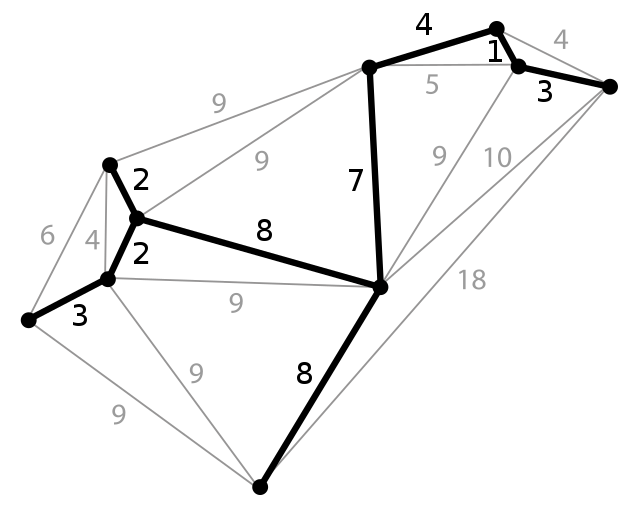
\includegraphics[width=.45\textwidth]{figures/640px-Minimum_spanning_tree.svg.png}
              \caption{Minimum cost spanning tree for a network}
          \end{figure}


    \item \textit{ Explain the difference between Prim's and Kruskal's Algorithm for finding minimum cost spanning tree with a small example graph.}\\

          The Main differences between the Two Algorithms are:
          \begin{enumerate}
              \item \textbf{Approach:} Prim's algorithm follows a \textit{greedy} approach where it starts from an arbitrary vertex and builds the tree by adding the next vertex with the lowest cost edge. On the other hand, Kruskal's algorithm is also a greedy approach, but it starts with the minimum edge and adds the next minimum edge which does not create a cycle.

              \item \textbf{Data structure:} Prim's algorithm uses a \textit{priority queue} to maintain the vertices with their minimum distance values, while Kruskal's algorithm uses a \textit{disjoint set data structure} to keep track of the connected components.

              \item \textbf{Complexity:} Prim's algorithm has a time complexity of $O(E\log V)$ for implementing with a priority queue, while Kruskal's algorithm has a time complexity of $O(E\log E)$ for implementing with a disjoint set data structure.

              \item \textbf{Connectivity:} Prim's algorithm generates a single tree rooted at the selected starting vertex, while Kruskal's algorithm generates multiple trees (i.e., forest) and later combines them into a single tree.

              \item \textbf{Graph type:} Prim's algorithm is more suitable for dense graphs (i.e., where $E$ is close to $V^2$), while Kruskal's algorithm works better for sparse graphs (i.e., where $E$ is much smaller than $V^2$).

              \item \textbf{Application:} Prim's algorithm is often used in network routing protocols, where finding the shortest path between two points is essential. On the other hand, Kruskal's algorithm is useful in applications like clustering, where finding the minimum cost connected subgraphs is required.

          \end{enumerate}
          \begin{table}[H]
              \begin{tabular}{|l|l|}
                  \hline
                  \textbf{Prim’s Algorithm}                                                                                                                                  & \textbf{Kruskal’s Algorithm}                                                                                                                                     \\ \hline
                  \begin{tabular}[c]{@{}l@{}}The tree that we are making or\\ growing always remains connected.\end{tabular}                                                 & \begin{tabular}[c]{@{}l@{}}The tree that we are making or growing usually \\ remains disconnected.\end{tabular}                                                  \\ \hline
                  \begin{tabular}[c]{@{}l@{}}Prim’s Algorithm grows a solution \\ from a random vertex adding the\\  next cheapest vertex to the existing tree.\end{tabular} & \begin{tabular}[c]{@{}l@{}}Kruskal’s Algorithm grows a solution from the\\  cheapest edge by adding the next cheapest\\  edge to the tree / forest.\end{tabular} \\ \hline
                  Prim’s Algorithm is faster for dense graphs.                                                                                                               & Kruskal’s Algorithm is faster for sparse graphs.                                                                                                                 \\ \hline
              \end{tabular}
          \end{table}
          \textbf{Example}: \\
          Consider the following graph:
          \begin{figure}[H]
              \centering
              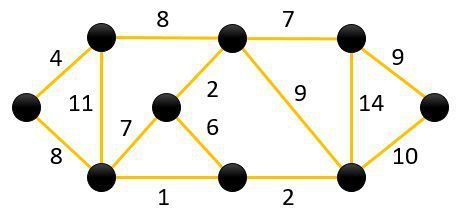
\includegraphics[width=.45\textwidth]{figures/Example.jpg}
              \caption{Example graph}
          \end{figure}

          \textbf{Prim's solution:} \\

          \begin{figure}[H]
              \centering
              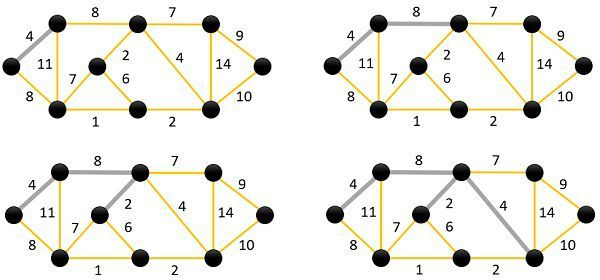
\includegraphics[width=.45\textwidth]{figures/Solution.jpg}
              \caption{Prim's solution}
          \end{figure}
          \begin{figure}[H]
              \centering
              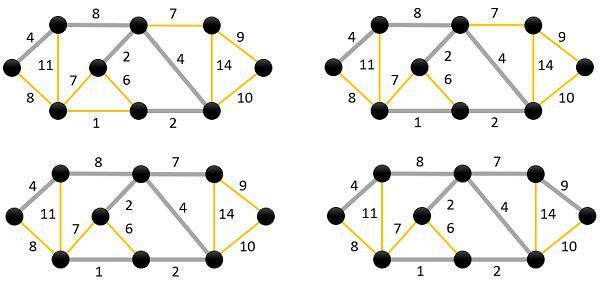
\includegraphics[width=.45\textwidth]{figures/Solution-part-2.jpg}
              \caption{Prim's solution}
          \end{figure}
          \textbf{Kruskal's solution: }\\

          \begin{figure}[H]
              \centering
              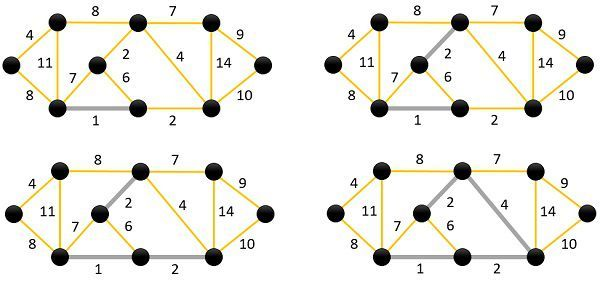
\includegraphics[width=.45\textwidth]{figures/Solution-kruskals.jpg}
              \caption{Kruskal's solution}
          \end{figure}

          \begin{figure}[H]
              \centering
              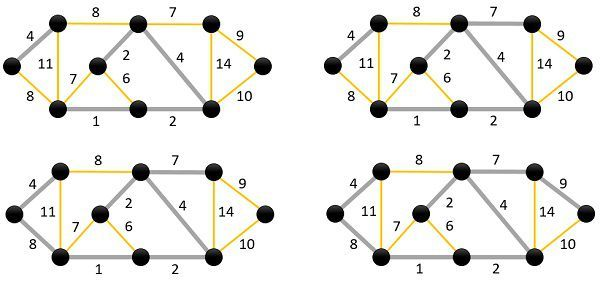
\includegraphics[width=.45\textwidth]{figures/Solution-kruskals-part-2.jpg}
              \caption{Kruskal's solution}
          \end{figure}

    \item \textit{ Which algorithmic strategy is used in Prim's algorithm. Explain that algorithmic strategy in brief.}\\

          \begin{itemize}
              \item Prim's algorithm for finding the minimum cost spanning tree uses a \textbf{Greedy approach}, which means that it makes the locally optimal choice at each step with the hope of finding a globally optimal solution.

              \item  The algorithm starts with a single vertex and keeps adding edges to the tree one by one, such that the tree grows gradually and remains connected at all times. At each step, the algorithm selects the edge with the minimum weight that connects a vertex in the tree to a vertex outside the tree. This process continues until all the vertices are included in the tree.

              \item The key idea behind the algorithm is to start with a small tree and gradually add vertices to it in a way that minimizes the total cost of the tree. The algorithm achieves this by always selecting the edge with the lowest weight that connects a vertex in the tree to a vertex outside the tree. By following this approach, the algorithm ensures that the tree is connected and has the minimum possible cost.

              \item Overall, Prim's algorithm is an efficient and widely used algorithm for finding the minimum cost spanning tree of a graph, especially when the graph is dense (i.e., has many edges).
          \end{itemize}
\end{enumerate}

\end{document}